%Conclusiones, Recomendaciones y Trabajos Futuros
\chapter{Resultados Experimentales}
\thispagestyle{empty}

En el presente capítulo se proecederá a explicar los resultados obtenidos a partir de las pruebas de las distintas maniobras cooperativas descritas en el Capítulo 6 en los distintos entornos de ensayos. Para estas pruebas, se empleó el sistema de comunicación reseñado en el Capítulo 5, el cual da paso a tres entornos, comunicación PC-PC, comunicación V2V y comunicación Vehículo-PC.\\

\par Estas pruebas se realizaron en la pista de TECNALIA \textit{Resarch \& Innovation}, tanto la versión real, como virtual (Figura \ref{fig:tecnaliap2}), en la cual se hizo un recorido completo, observando el comportamiento de los controladores en todo momento. Las pruebas experimentales comprenden exclusivamente la maniobra de ACC sin integración del Control Lateral.   

%%%%%%
\section{Comunicación PC - PC}
%%%%%%
En esta prueba se evalúa el desempeño de los controladores en cada maniobra, empleando dos computadoras conectadas a una misma red WLAN, en las cuales se pone en marcha el simulador Dynacar, junto con el Visor 3D, donde se puede observar el vehículo simulado en la computadora con la cual se está comunicando. En la Figura \ref{fig:vlidseg}, se puede apreciar un ejemplo de lo que se observa en ambas computadoras, donde se tienen los vehículos simulados en dichas PC (carros naranjas) y los vehículos simulados en la otra PC (carros azules).\\   

\begin{figure}[H]
 \centering
  \subfloat[Simulador de la PC correspondiente al vehículo seguidor]{
   \label{fig:a}
    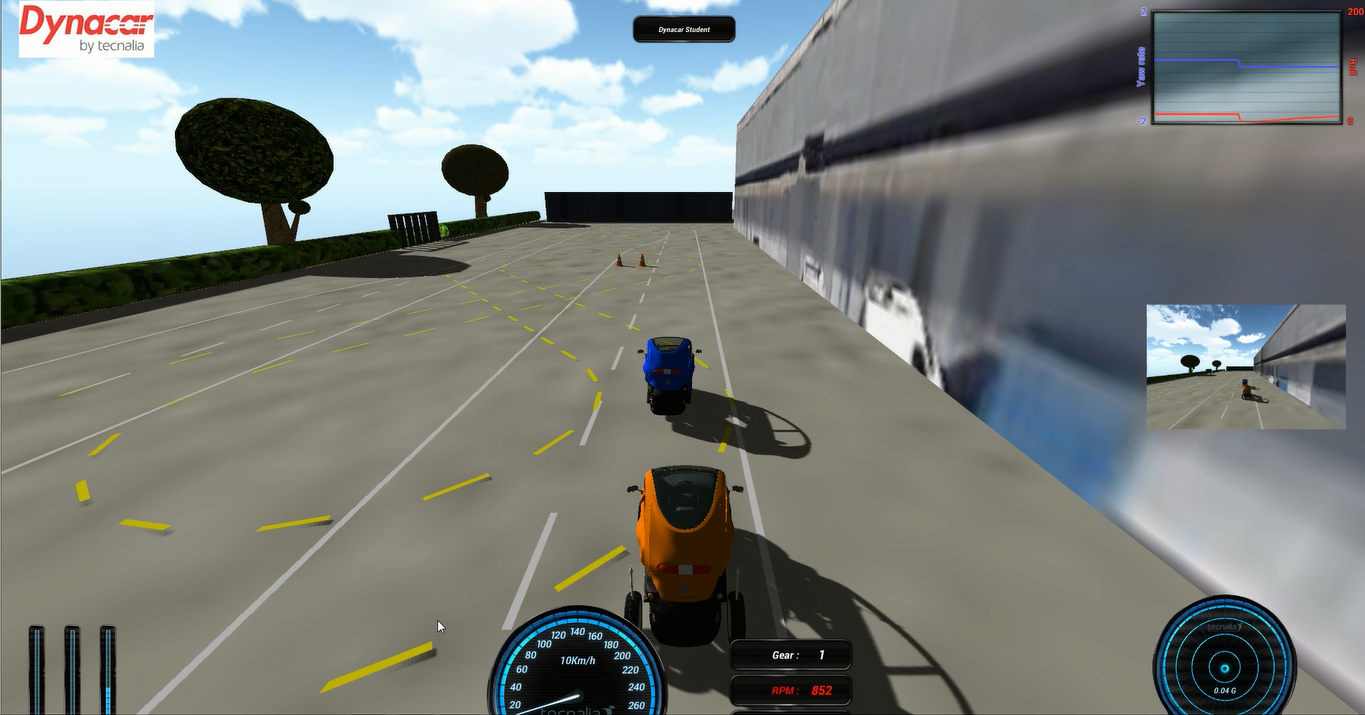
\includegraphics[scale=0.215]{Imagenes/vseg}}
  \subfloat[Simulador de la PC correspondiente al vehículo líder]{
   \label{fig:v}
    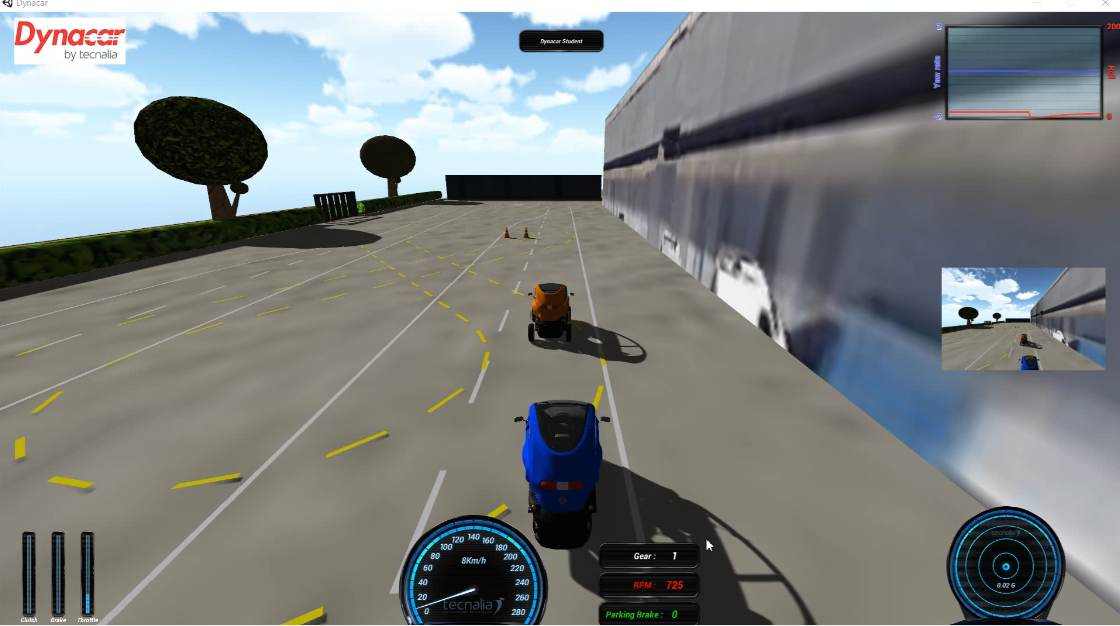
\includegraphics[scale=0.25]{Imagenes/vlid}}
 \caption{Vista del simulador en ambas computadoras}
 \label{fig:vlidseg}
\end{figure}

\subsection{ACC}
Para la prueba del ACC se modificó la velocidad del vehículo líder a medida que avanzaba, simulando de esta forma lo más posible el comportamiento de un vehículo real, con lo cual el carro seguidor tiene que ir ajustando su velocidad, guardando cierta distancia. En este caso el vehículo seguidor comienza por detrás de la distancia de seguridad, teniendo que acercarse a la misma, y luego arrancar una vez lo haga el líder. Un ejemplo de esta situación puede ser encontrado en la figura \ref{fig:accej}. Además debido a las características de la pista, solo son permitidas velocidades bajas, por lo cual los vehículos no exceden los 20 km/h.\\

\begin{figure}[H]
	\centering
		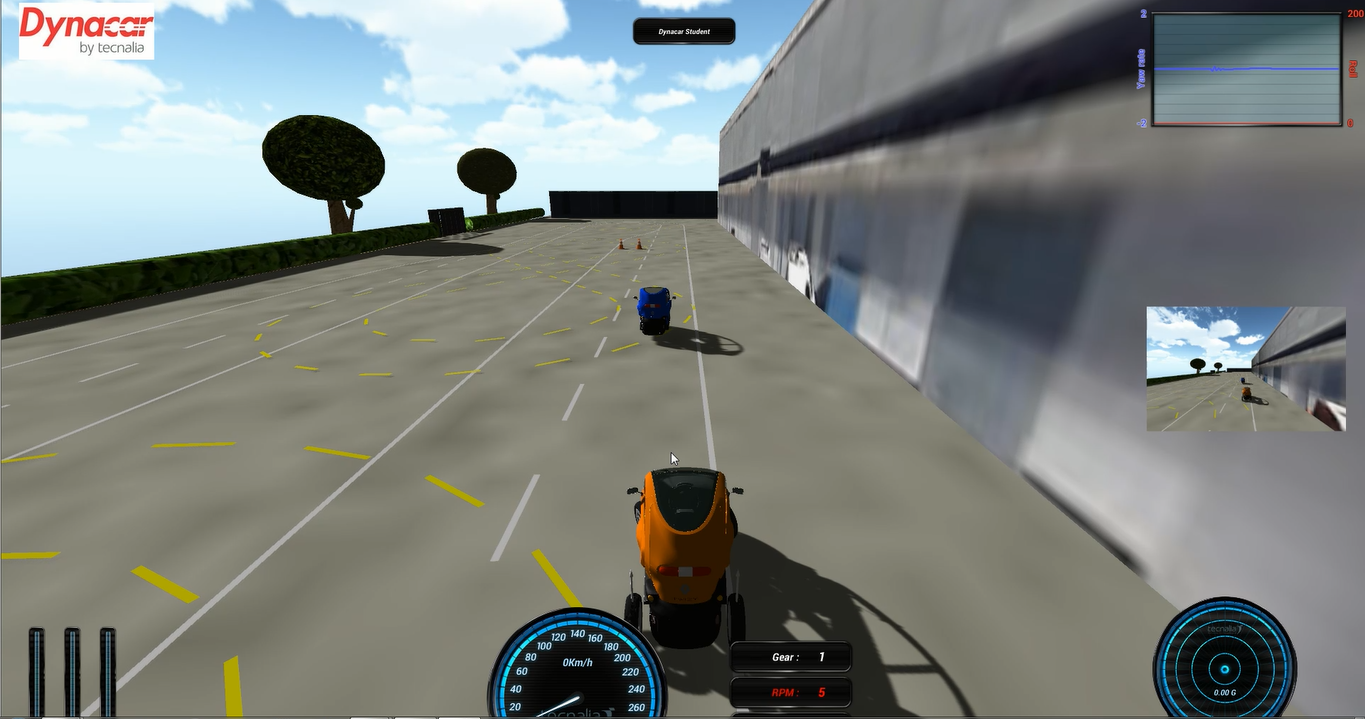
\includegraphics[scale=0.35]{Imagenes/accej}
		\caption{Ejemplo del vehículo seguidor comenzando por detrás de la distancia de seguridad.}
		\label{fig:accej}
\end{figure}	

\par Como se puede apreciar en la Figuras \ref{fig:velacc} y \ref{fig:disacc}, el vehículo seguidor realiza un pequeño movimiento, hasta encontrarse sobre la distancia de referencia, para luego arrancar junto al vehículo líder, apegándose a la velocidad de referencia, con un pequeño error menor al 3 \%, a execpción del tramo final, donde se puede ver que el vehículo aceleró, al disminuirse la referencia de distancia, aún así es un valor pequeño, que produce un error menor al 5 \% con respecto a la distancia de seguridad.\\
\begin{figure}[H]
	\centering
		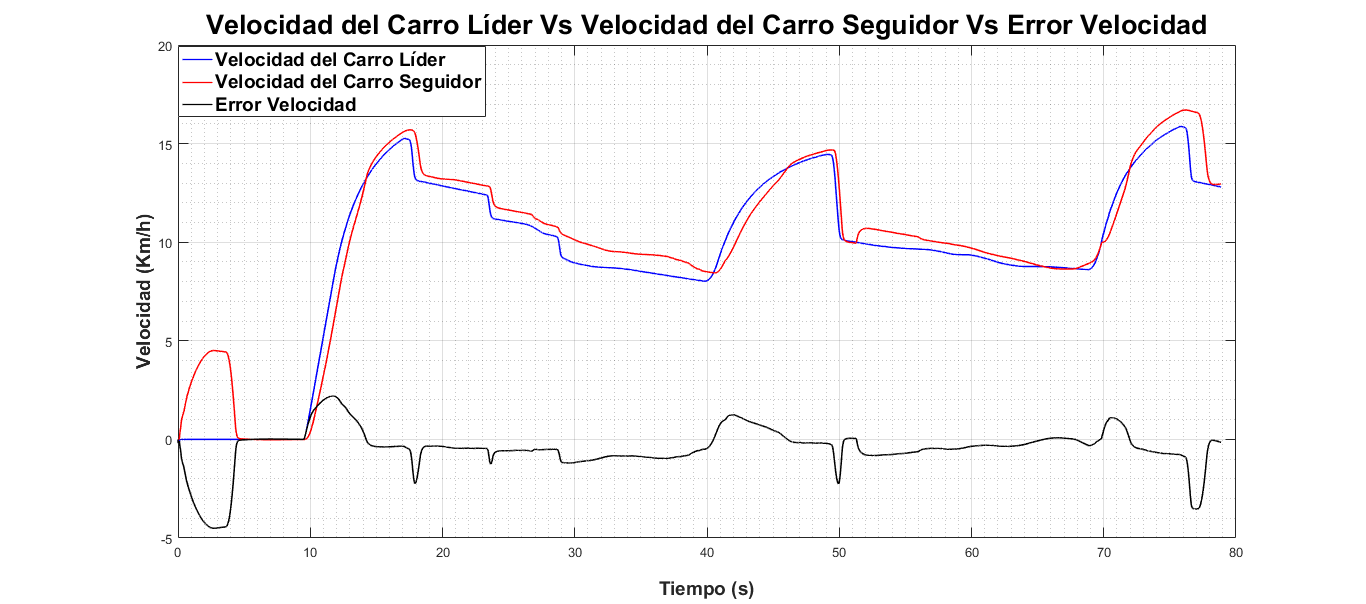
\includegraphics[scale=0.35]{Imagenes/velacc}
		\caption{Gráfica de la velocidad de los vehículos}
		\label{fig:velacc}
\end{figure}	

\begin{figure}[H]
	\centering
		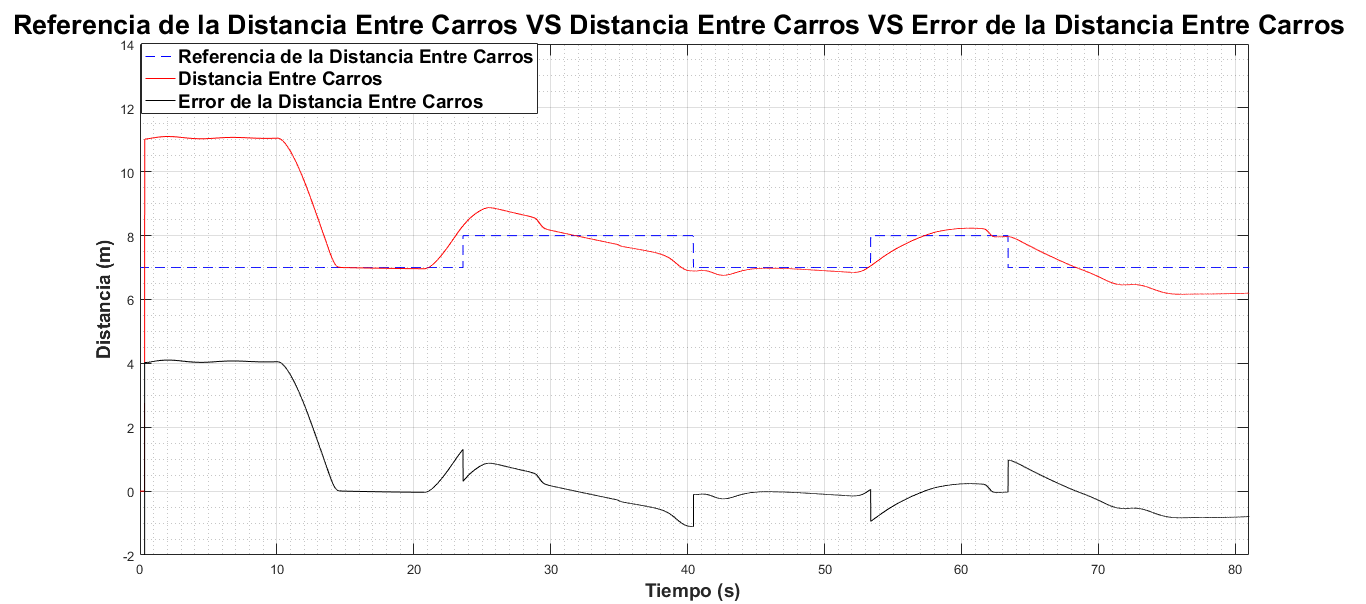
\includegraphics[scale=0.35]{Imagenes/disacc}
		\caption{Gráfica del error de la distancia de los vehículos}
		\label{fig:disacc}
\end{figure}	

%%%%%%
\subsection{Control Lateral}
%%%%%%
Para la prueba del Control Lateral se fijaron las posiciones iniciales de los vehículos de tal forma que el carro seguidor tuviese que ajustar en pequeña medida su posición con respecto a la del líder. Así pues, en la Figura \ref{fig:rutacl} se puede observar que el vehículo seguidor sigue casi a la perfección la ruta del vehículo líder, encontrando un mayor error, al final de las curvas, sin embargo sigue siendo una diferencia muy pequeña.  \\

\begin{figure}[H]
 \centering
  \subfloat[Gráfica de la ruta seguida por los vehículos]{
   \label{fig:vcl}
    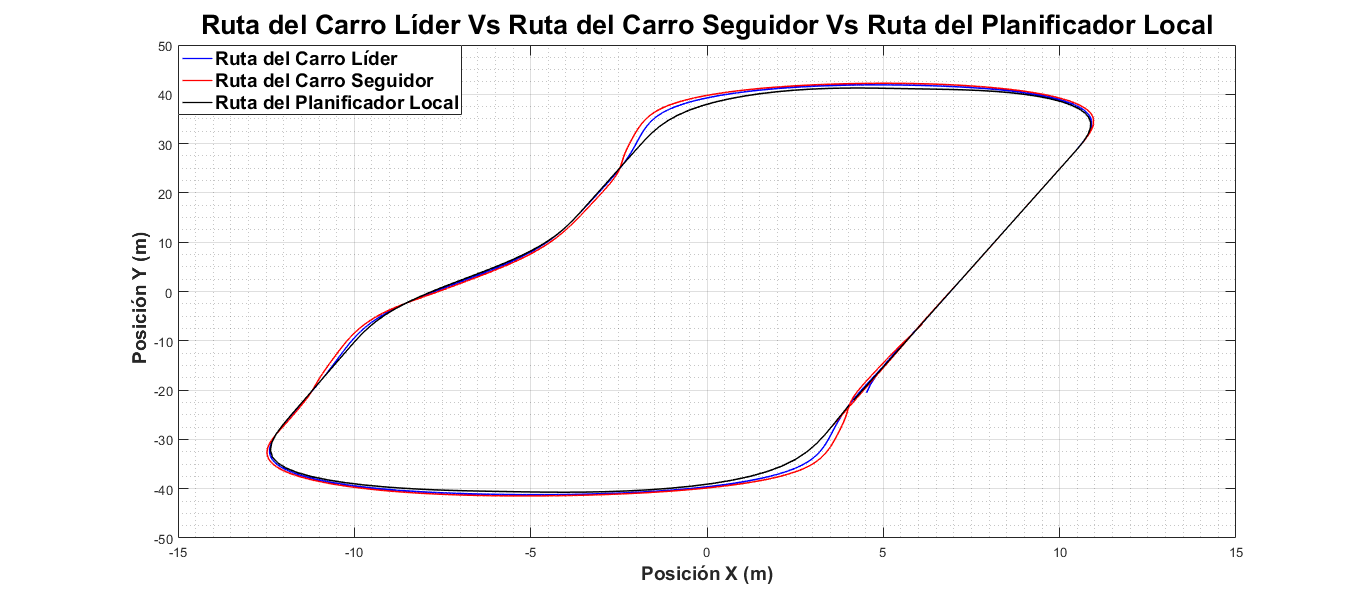
\includegraphics[scale=0.25]{Imagenes/rutacl}}
  \subfloat[Ruta seguida por los vehículos en Dynacar]{
   \label{fig:tecnaliap}
    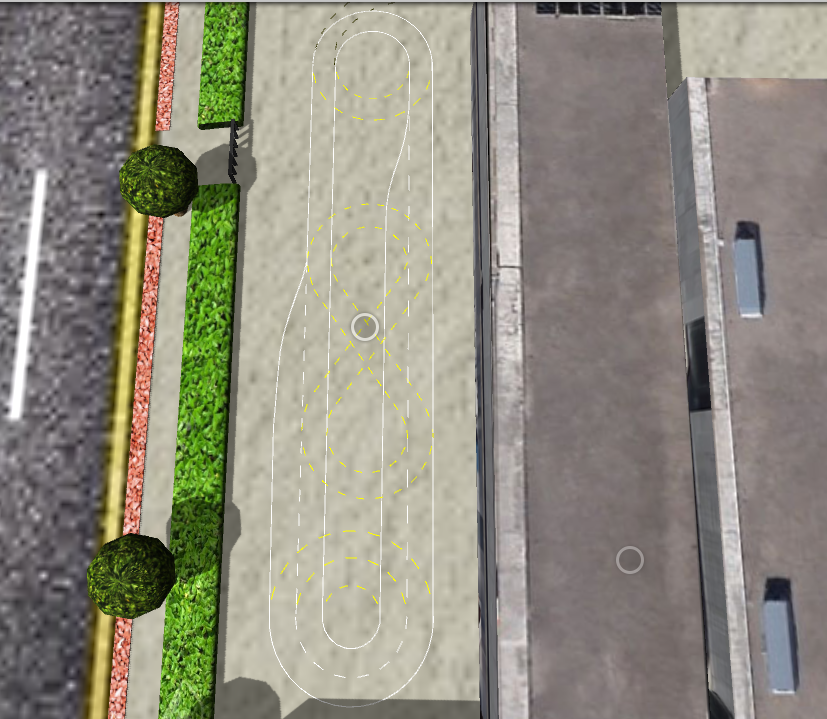
\includegraphics[scale=0.25]{Imagenes/tecnaliap}}
 \caption{Ruta establecida para la prueba de Control Lateral con comunicación PC - PC}
 \label{fig:rutacl}
\end{figure}

\par Para un mejor análisis, a continuación se presentan las graficas del error lateral (Figura \ref{fig:elcl})  y angular (Figura \ref{fig:eacl}) de los vehículos, donde se puede apreciar que el máximo error que se presenta con respecto al ángulo es de 20 grados, y con lateral de 55 cm, que corresponden a la primera curva. Mientras que, para el cambio de carril se tienen unos errores de 5 grados y 15 cm, y para la segunda curva, 15.1 grados, y 48 cm.\\

\begin{figure}[H]
	\centering
		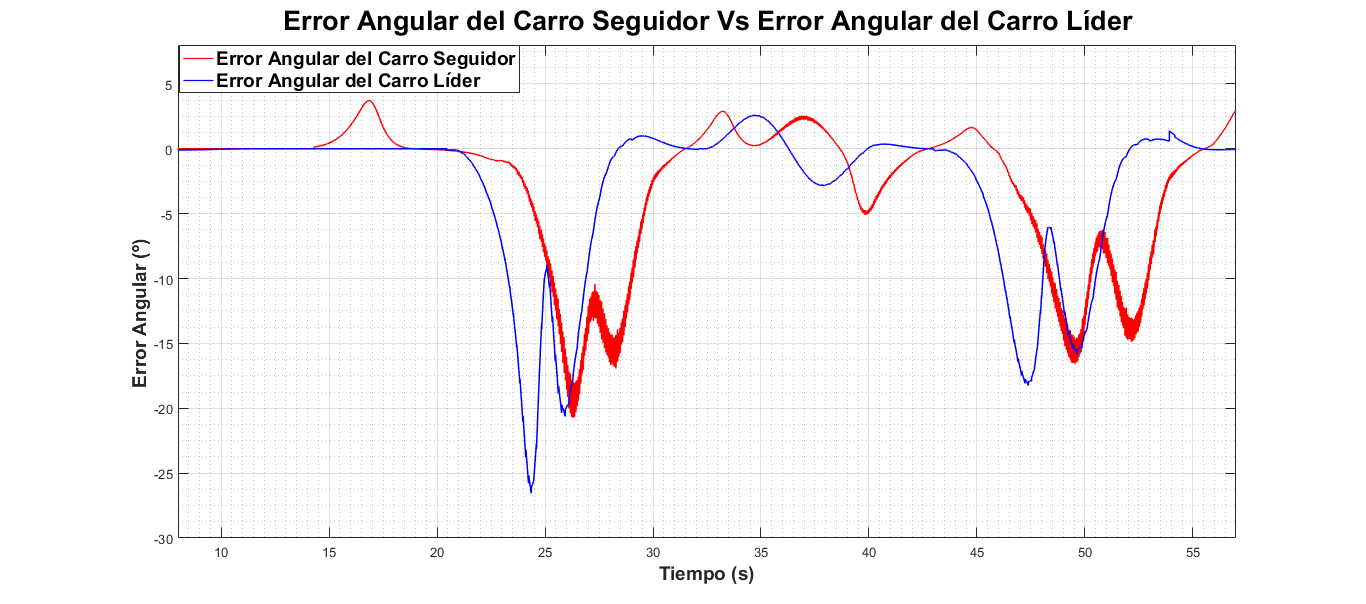
\includegraphics[scale=0.35]{Imagenes/eacl}
		\caption{Gráfica del error angular de los vehículos}
		\label{fig:eacl}
\end{figure}	

\begin{figure}[H]
	\centering
		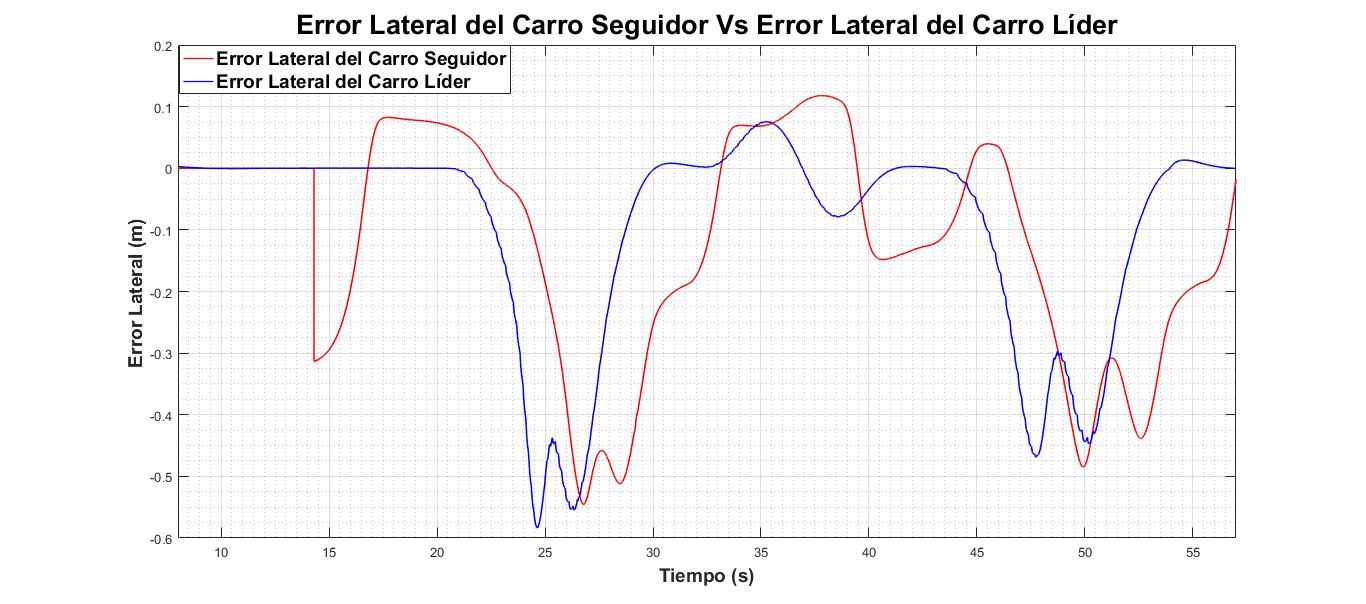
\includegraphics[scale=0.35]{Imagenes/elcl}
		\caption{Gráfica del error lateral de los vehículos}
		\label{fig:elcl}
\end{figure}	

%%%%%%
\subsection{\textit{Stop and Go}}
%%%%%%
Para la maiobra de \textit{Stop and Go}, se realizó la misma prueba, que la presentada en la sección 6.3, obteniendo como resultado que el vehículo seguidor, mantuvo la referencia de velocidad, frenando a 6.5 m de distancia, excediendo 50 cm, la distancia de referencia.\\
\begin{figure}[H]
	\centering
		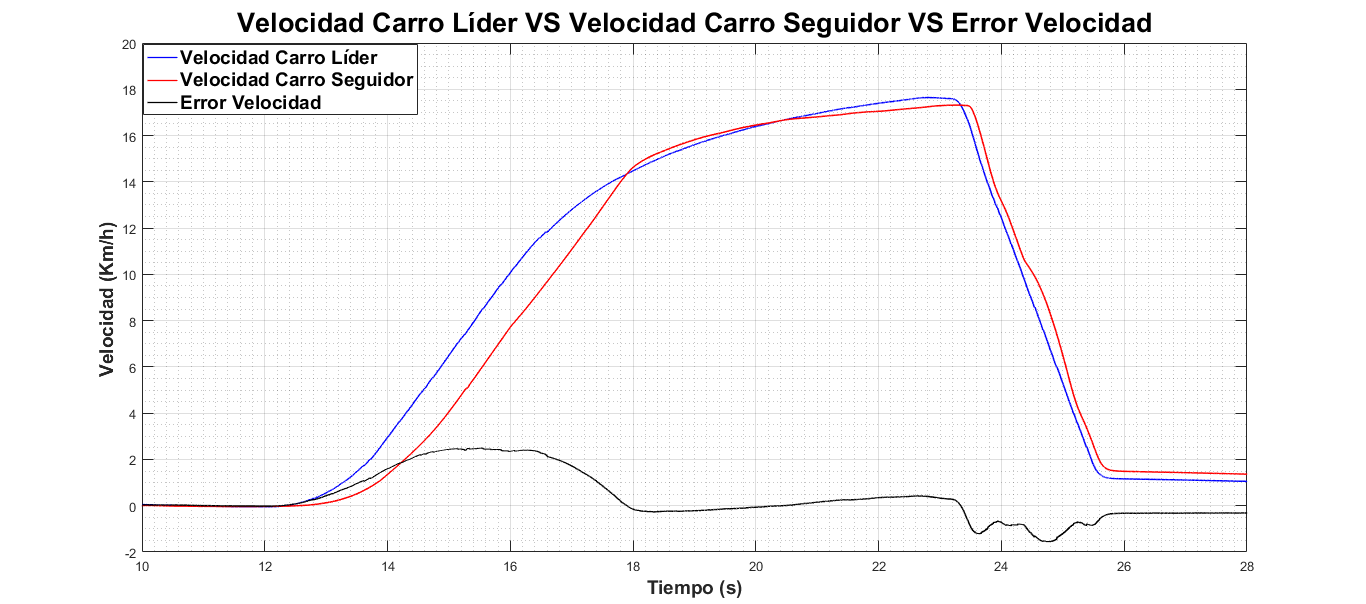
\includegraphics[scale=0.35]{Imagenes/velstg1}
		\caption{Gráfica de la velocidad de los vehículos}
		\label{fig:velstg1}
\end{figure}	

\begin{figure}[H]
	\centering
		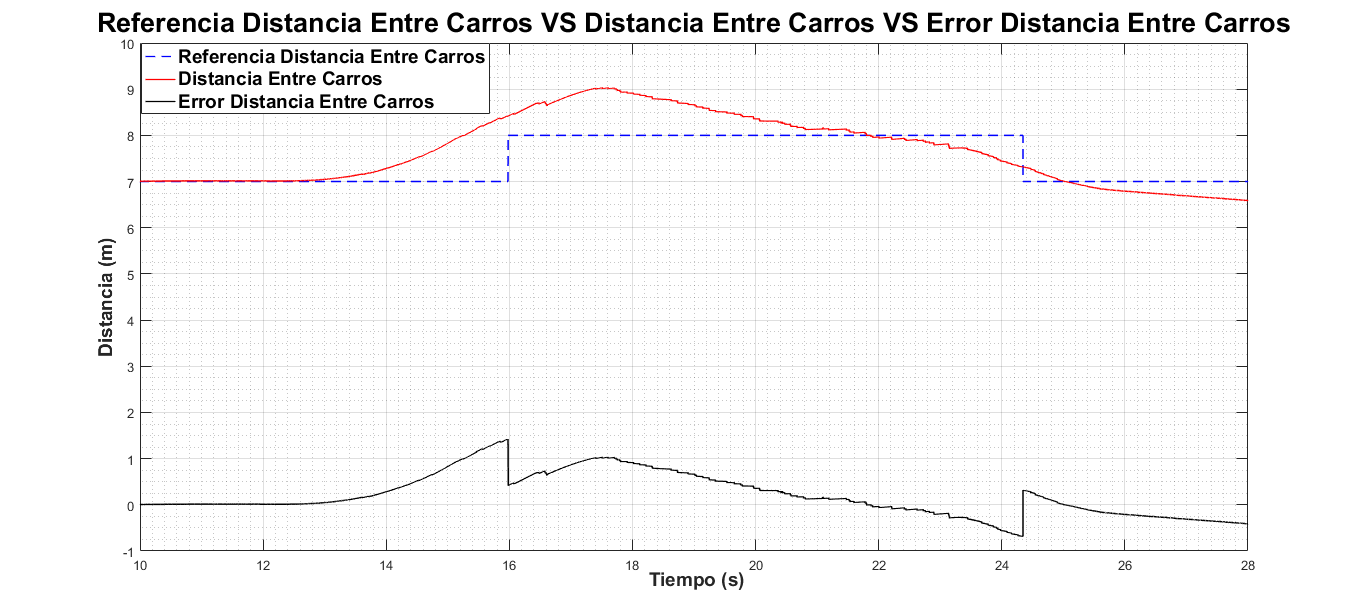
\includegraphics[scale=0.35]{Imagenes/diststg1}
		\caption{Gráfica del error de la distancia de los vehículos}
		\label{fig:diststg1}
\end{figure}	

%%%%%%
\subsection{ACC con Control Lateral}
%%%%%%

Para la prueba del ACC con Control Lateral, se combinó la forma de iniciar de ambas pruebas, es decir a una distancia mayor que la de referencia, y en un canal distinto. En cuanto longitudinal, se puede apreciar, en la Figura \ref{fig:veacl}, que el vehículo seguidor, mantiene la velocidad del líder, presentando los mismos errores que si se estuviese usando solo este controlador, De la misma forma, en la Figura \ref{fig:diacl}, se observa como el vehículo sigue a la referencia, presentando un error máxmo al estabilizarse de 20 cm.\\   

\begin{figure}[H]
	\centering
		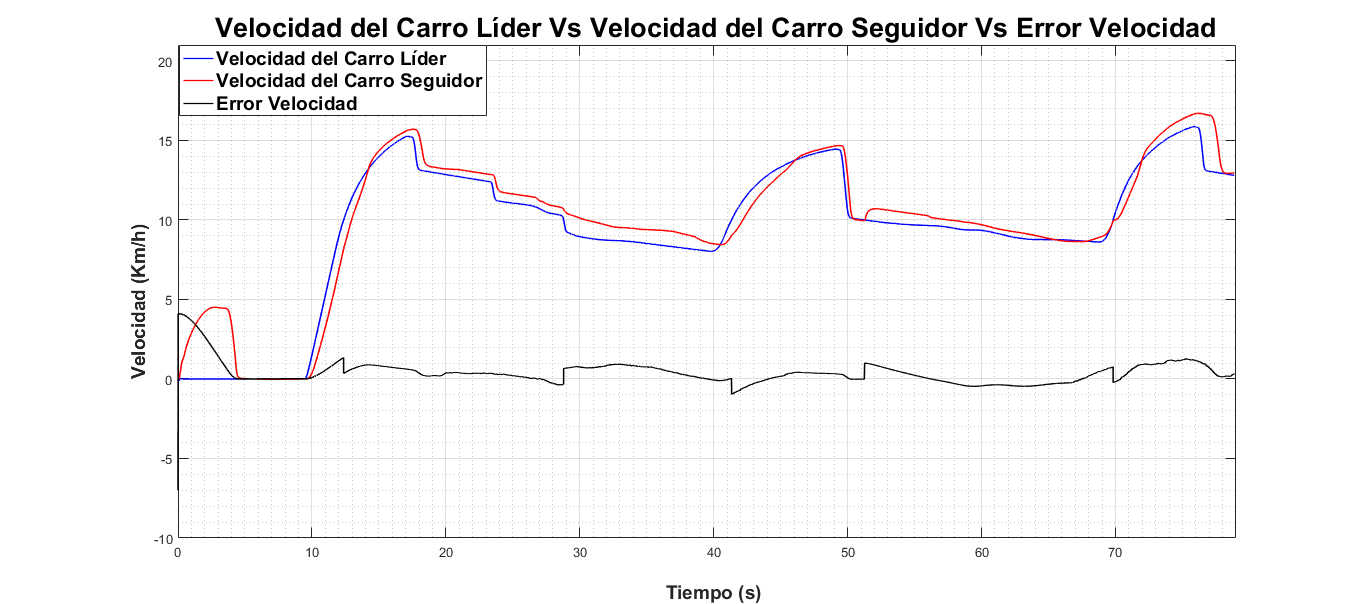
\includegraphics[scale=0.35]{Imagenes/veacl}
		\caption{Gráfica de la velocidad de los vehículos}
		\label{fig:veacl}
\end{figure}	

\begin{figure}[H]
	\centering
		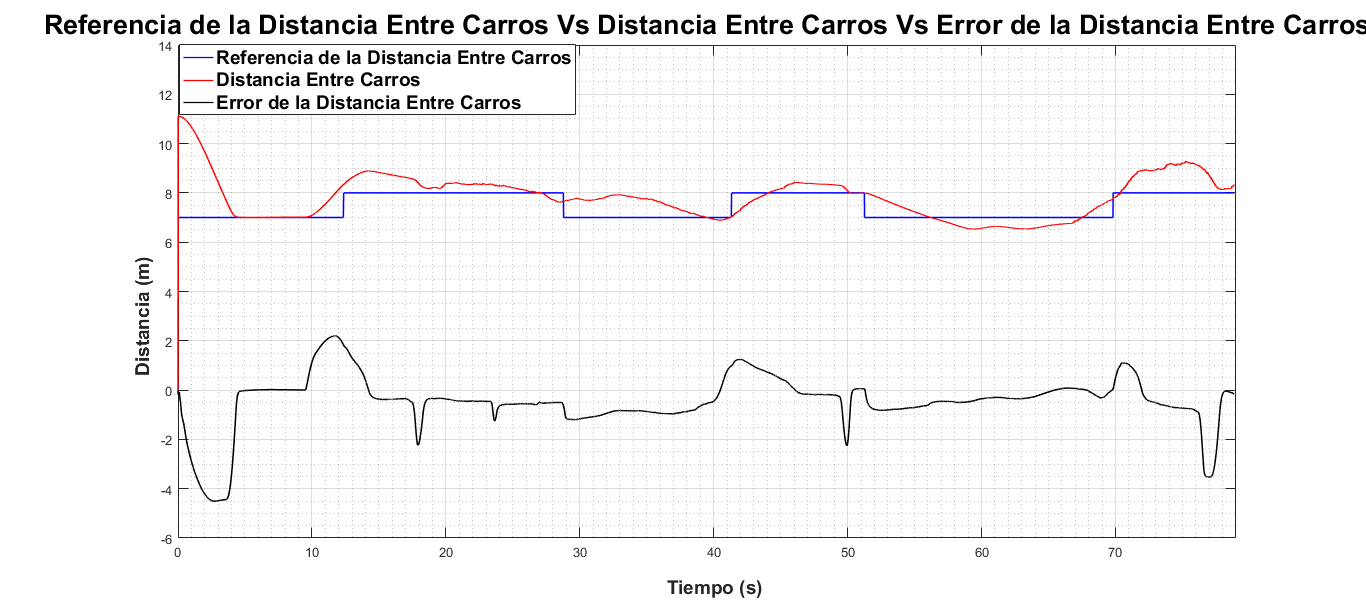
\includegraphics[scale=0.35]{Imagenes/diacl}
		\caption{Gráfica del error de la distancia de los vehículos}
		\label{fig:diacl}
\end{figure}	

\par En lo que respecta a la parte lateral, se puede apreciar que, al igual que la Figura \ref{fig:rutacl}, la Figura \ref{fig:rutaccl}, muestra que las rutas seguida por los vehículos, es muy parecida, diferenciándose, un poco al momento de realizar las curvas.Sin embargo, es una dieferencia que se puede considerar despreciable.\\ 

\begin{figure}[H]
 \centering
  \subfloat[Gráfica de la ruta seguida por los vehiculos]{
   \label{fig:vhaccl}
    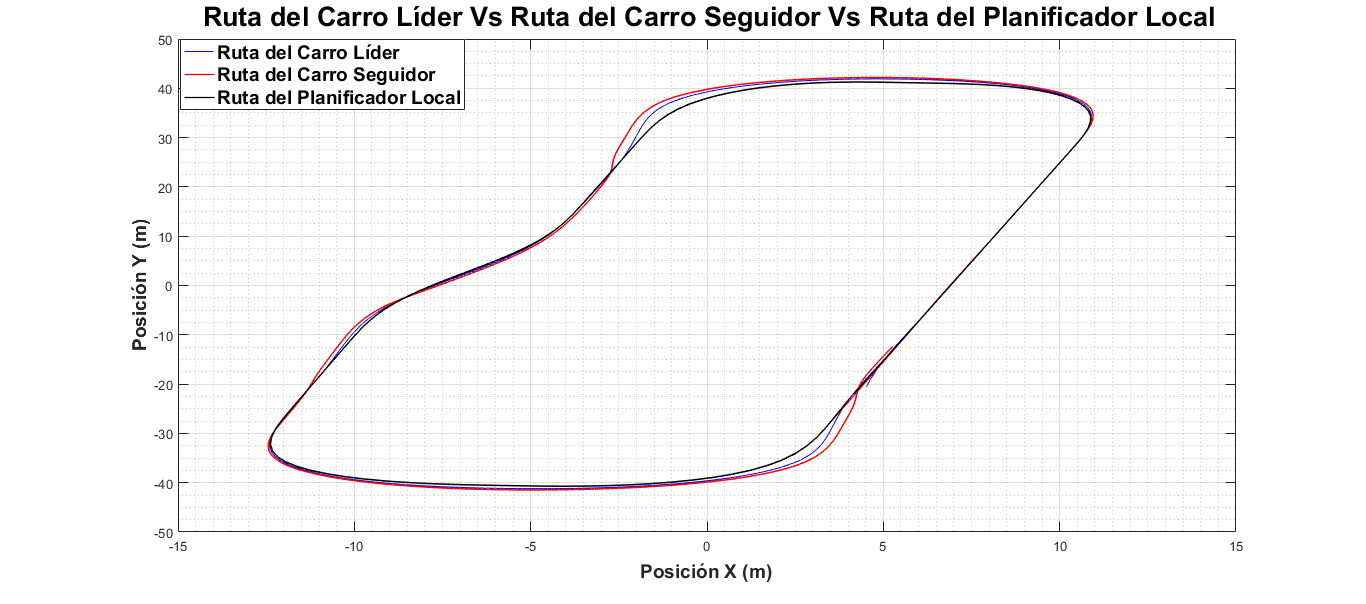
\includegraphics[scale=0.25]{Imagenes/rutaaccl}}
  \subfloat[Ruta seguida por los vehículos en Dynacar]{
   \label{fig:dyaccl}
    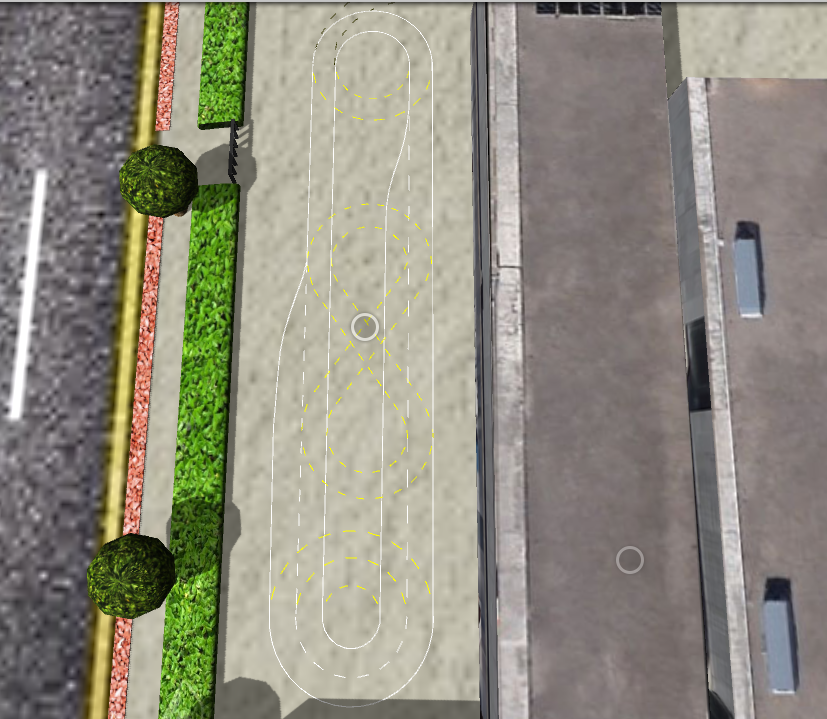
\includegraphics[scale=0.25]{Imagenes/tecnaliap}}
 \caption{Ruta establecida para la prueba del ACC con Control Lateral con comunicación PC - PC}
 \label{fig:rutaccl}
\end{figure}

\par Para comprobar esta similitud, se pueden observar las Figuras \ref{fig:eaacl} y \ref{fig:elacl}, las cuales muestran el comportamiento de los errores angular y lateral de los vehículos, en la que se observa que los errores máxmos son presentados en las curvas, y poseen un valor de, 18 grados y 52 cm, para la curva 1, y 17 grados y 42 cm, para la curva 2, mostrando así un buen desempeño, ante el uso de comunicaciones. \\

\begin{figure}[H]
	\centering
		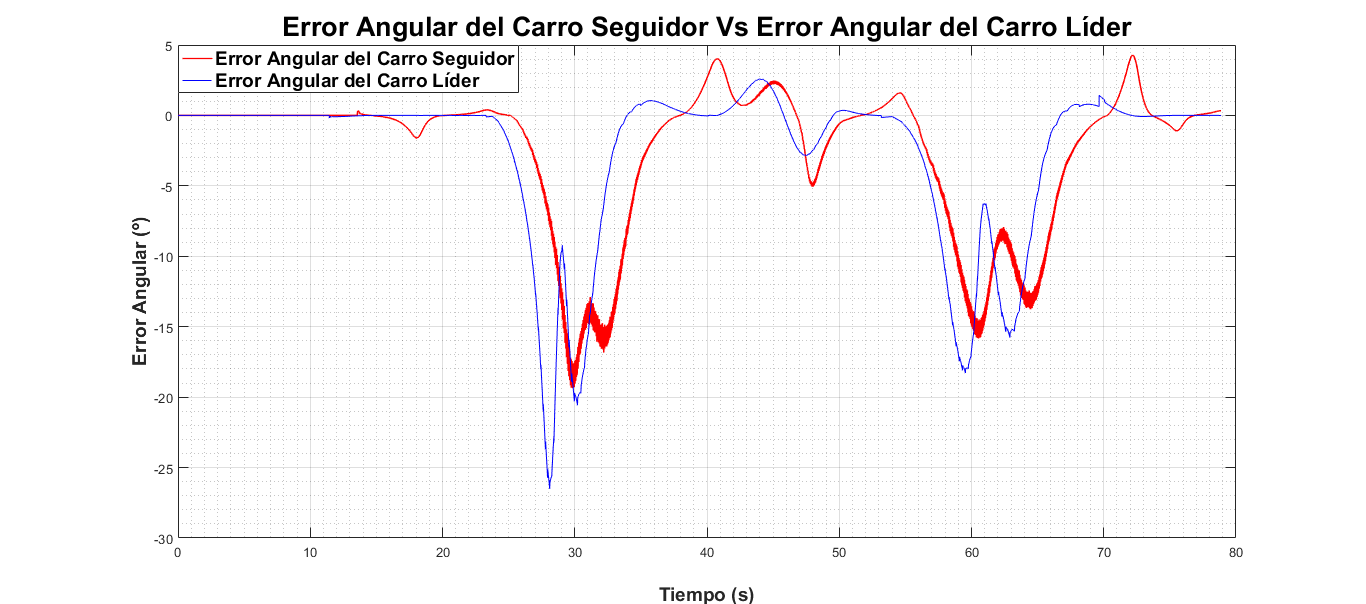
\includegraphics[scale=0.35]{Imagenes/eaacl}
		\caption{Gráfica del error angular de los vehículos}
		\label{fig:eaacl}
\end{figure}	

\begin{figure}[H]
	\centering
		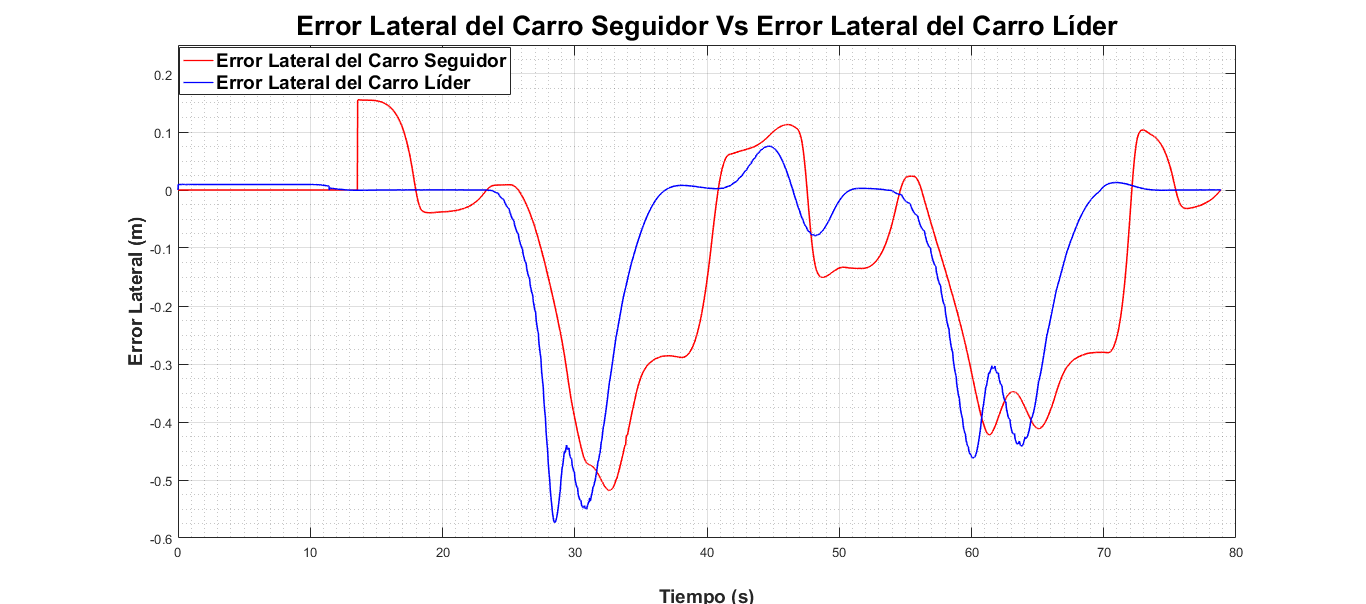
\includegraphics[scale=0.35]{Imagenes/elacl}
		\caption{Gráfica del error lateral de los vehículos}
		\label{fig:elacl}
\end{figure}	

\section{Comunicación Vehículo - Vehículo, V2V}
La presente sección evalúa el desempeño, del sistema de comuncaciciones junto con el control longitudinal para las maniobras de ACC y \textit{Stop and Go} en los vehículos reales (Figura \ref{fig:accreal}). Para esta prueba se empleó una comunicación unidireccional, en la que el vehículo líder envía su posición y velocidad al vehículo seguidor, el cual realiza las acciones necesarias. Para la misma se emplea una tasa de envío de 10 ms.\\

\begin{figure}[H]
	\centering
		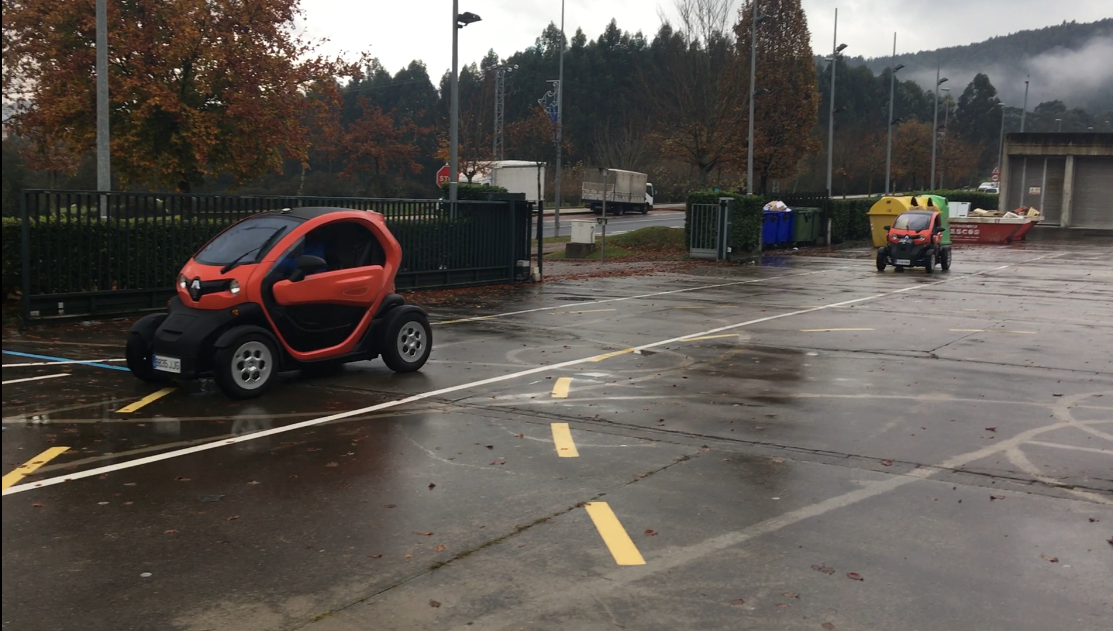
\includegraphics[scale=0.45]{Imagenes/accreal}
		\caption{Vehículos Twizy realizando la maniobra de ACC}
		\label{fig:accreal}
\end{figure}	

%%%%%%
\subsection{ACC}
%%%%%%
Al igual que las pruebas anteriores se varió la velocidad del vehículo líder, buscando que el vehículo seguidor mantuviese la referencia de velocidad y distancia. El compotamiento del vehículo puede ser observado en las Figuras \ref{fig:velrea} y \ref{fig:distrea} , donde se observa similitud en la comprativa de velocidades, a diferencia de la distancia, la cual posee un mayor error, llegando a estar sobre los 14 m de diferencia, defecto que se debe al cambio de velocidad presente al momento de tomar la curva, sumado al hecho, de que el cálculo de la distancia es una aproximación a una recta, lo que implica que en tramos curvos se pueda presentar un error mayor, a pesar de esto, el controlador mustra una respuesta satisfactoria en el resto del recorrido. \\  
\begin{figure}[H]
	\centering
		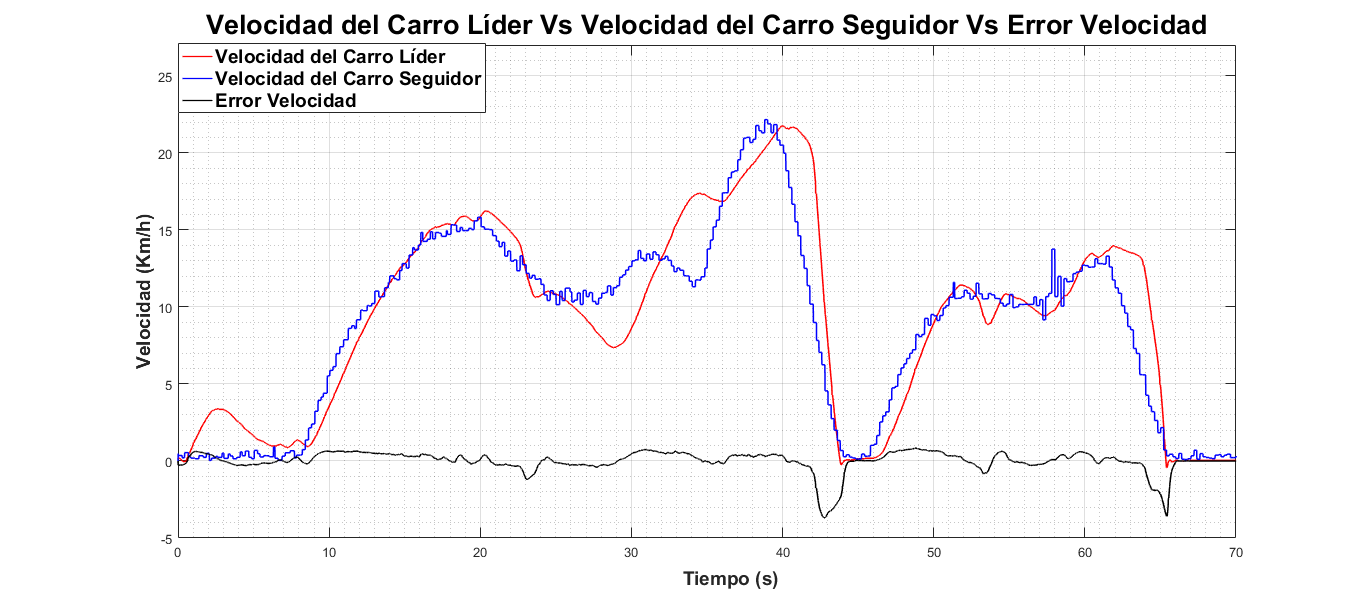
\includegraphics[scale=0.35]{Imagenes/velrea}
		\caption{Gráfica de la velocidad de los vehículos}
		\label{fig:velrea}
\end{figure}	

\begin{figure}[H]
	\centering
		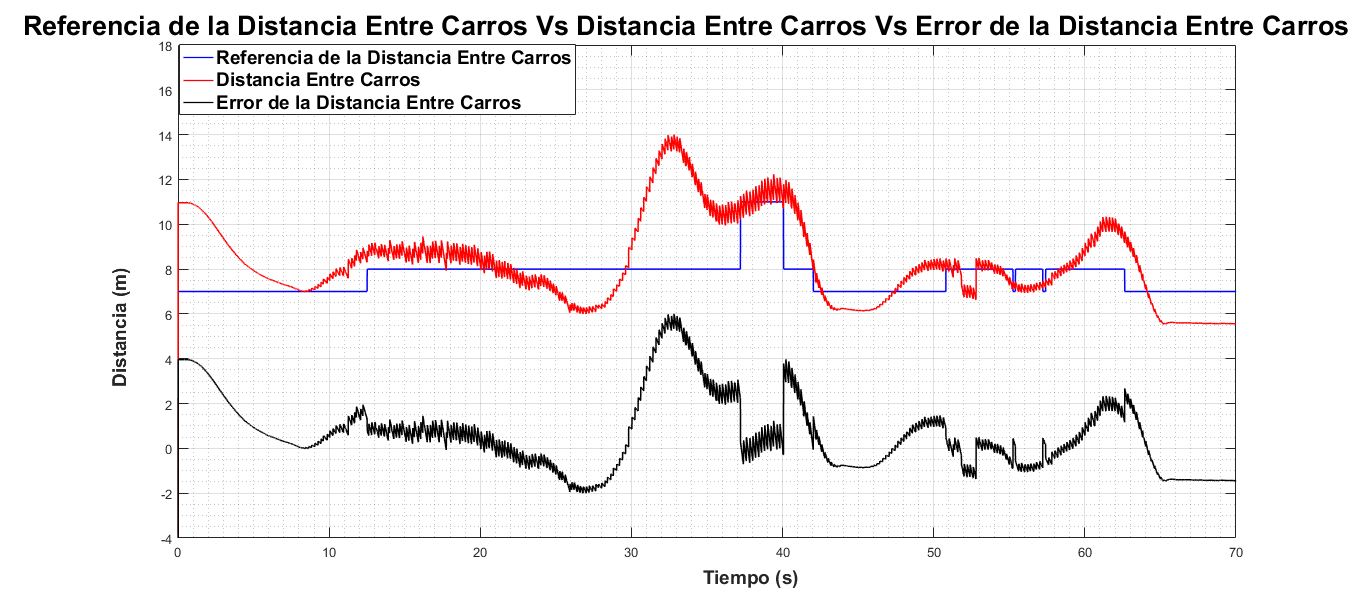
\includegraphics[scale=0.35]{Imagenes/distrea}
		\caption{Gráfica del error de la distancia de los vehículos}
		\label{fig:distrea}
\end{figure}	


%%%%%%
\subsection{\textit{Stop and Go}}
%%%%%%
En la Figura \ref{fig:velreastg} se puede apreciar como el vehículo seguidor mantiene la velocidad, con la diferencia que el frenado lo empieza a realizar 5 s depués que el vehículo líder, sobrepasando de esta forma la distancia de segurdad en 1 m, como es observardo en la Figura \ref{fig:distreastg}, en la cual además se ve como se mantiene un error de 1 m sobre la referencia.\\ 
\begin{figure}[H]
	\centering
		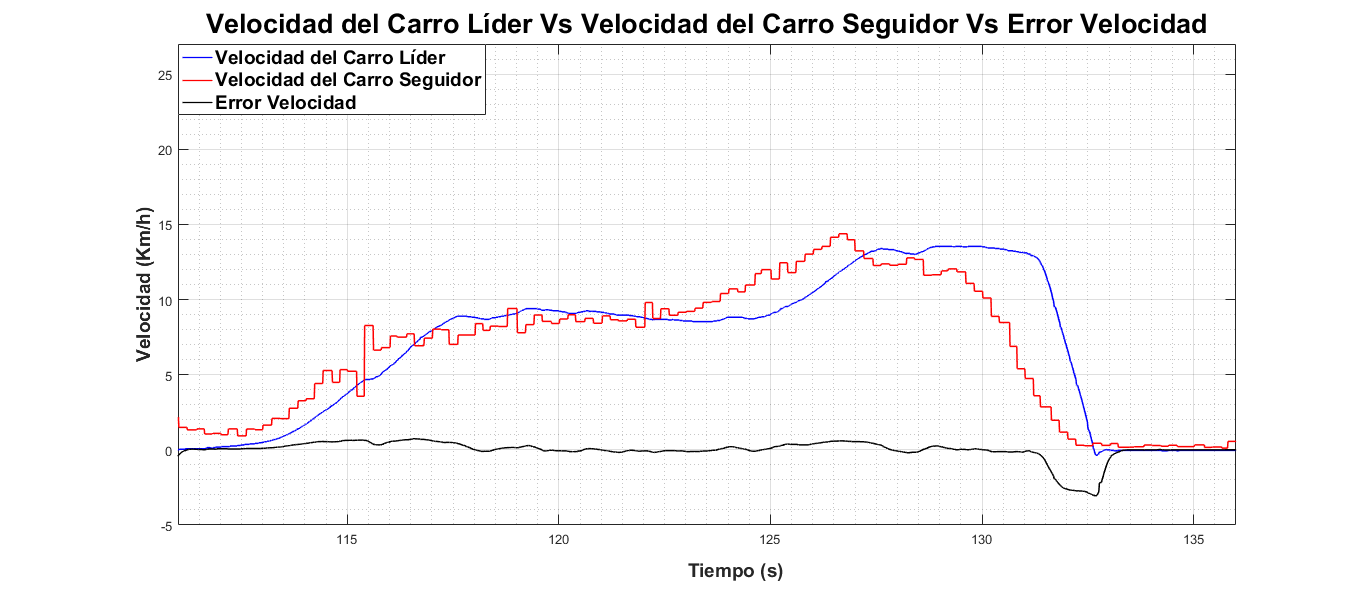
\includegraphics[scale=0.35]{Imagenes/velreastg}
		\caption{Gráfica de la velocidad de los vehículos}
		\label{fig:velreastg}
\end{figure}	

\begin{figure}[H]
	\centering
		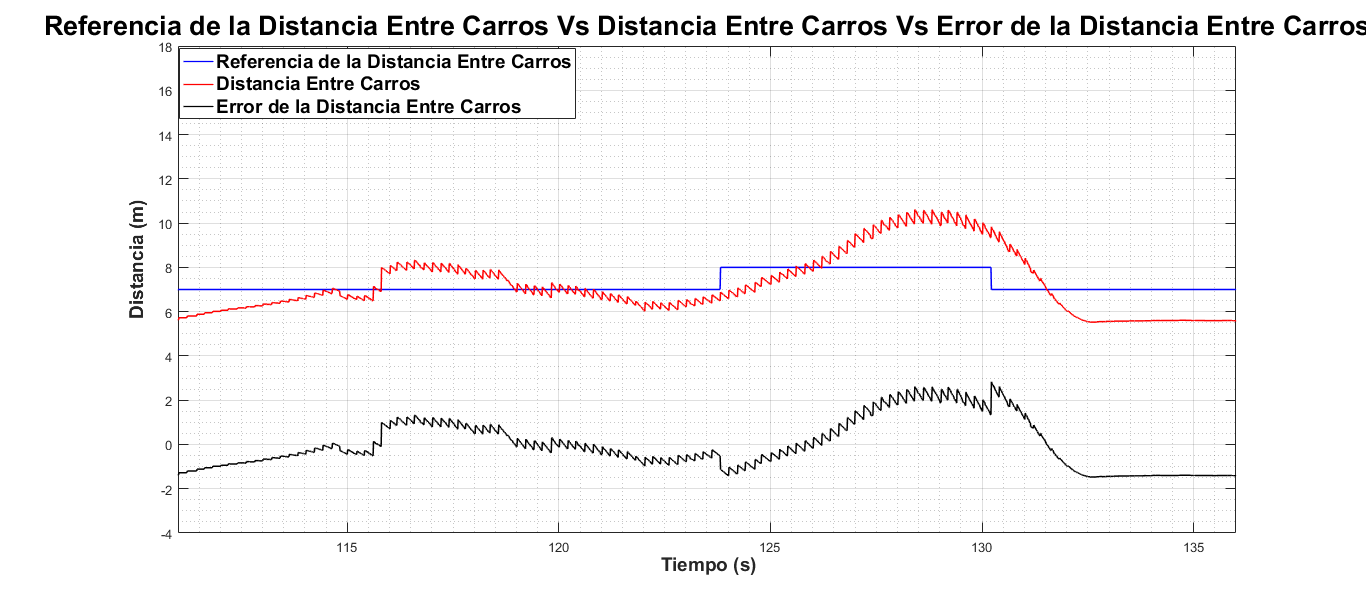
\includegraphics[scale=0.35]{Imagenes/distreastg}
		\caption{Gráfica del error de la distancia de los vehículos}
		\label{fig:distreastg}
\end{figure}	


\section{Comunicación Vehículo - PC}

En este escenario se probaron, tanto el controlador para las maniobras de ACC y \textit{Stop and Go}, como el sistema de comunicación, para la conexión entre un vehículo real, y un vehículo virtual, el cual es simulado a través de Dynacar. Además, se busca poder observar el vehículo real en el Visor 3D, y de esta forma tener un monitoreo completo del mismo en la computadora (Figura \ref{fig:cardynacar}).\\

\begin{figure}[H]
 \centering
  \subfloat[Vehículo realizando la maniobra la maniobra de ACC, con el carrro virtual]{
   \label{fig:dynacar}
    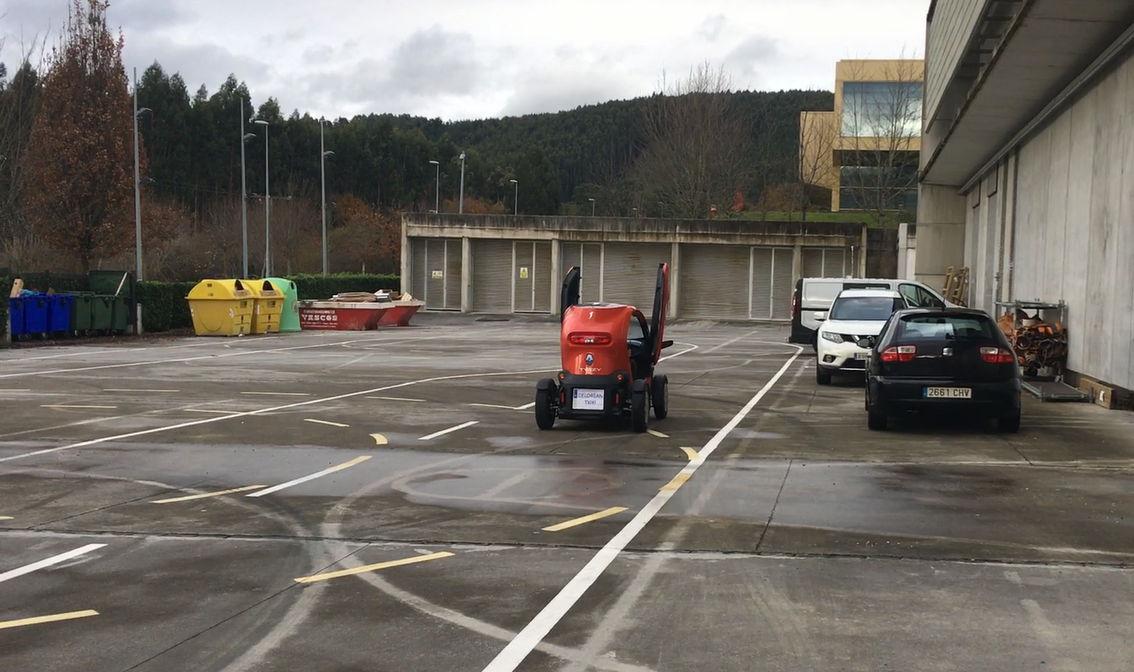
\includegraphics[scale=0.25]{Imagenes/dynacar}}
  \subfloat[PC donde se muestran tanto el vehículo virtual, como el real]{
   \label{fig:cardyna}
    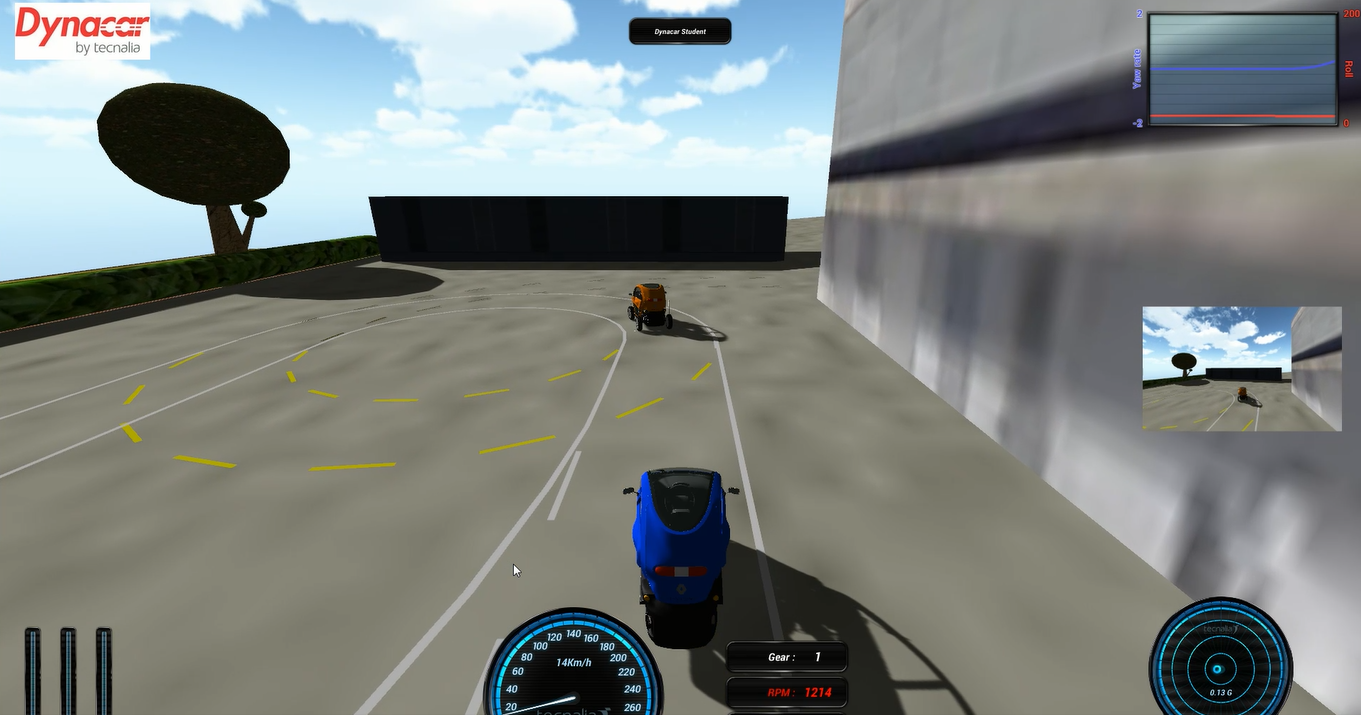
\includegraphics[scale=0.23]{Imagenes/cardyna}}
 \caption{Ejemplo de la comunicación Vehículo - PC}
 \label{fig:cardynacar}
\end{figure}

\par Debido al uso del carro real y de una comunicación bidireccional, la tasa de envío se cambió a 50 ms, buscando el mejor funcionamiento del vehículo real, el cual cumple la función de seguidor, siendo el virtual, el líder.

%%%%%%
\subsection{ACC}
%%%%%%
En la Figura \ref{fig:velacccs} se puede observar el correcto funcionamiento del controlador longitudinal, al tener seguir casi a la perfección la velocidad del carro líder, teniendo una respuesta rápida, que además se ve complementado por el echo del vehículo acelerar de forma correcta para alcanzar la distancia de referencia, antes de que el carro líder arranque. Para el completo análisis, en la Figura \ref{fig:distacccs}, se aprecia como efectivamente el vehículo se acerca hasta llegar a la distancia de seguridad, y posteriormente mantiene de buena forma la distancia referencia, a excepción del tramo final, correspondiente al frenado del vehículo, el cual termina excediendo la distancia de seguridad por 3 m, mostrando el mayor error a la hora de realizar esta acción entre las pruebas realizadas.\\
\begin{figure}[H]
	\centering
		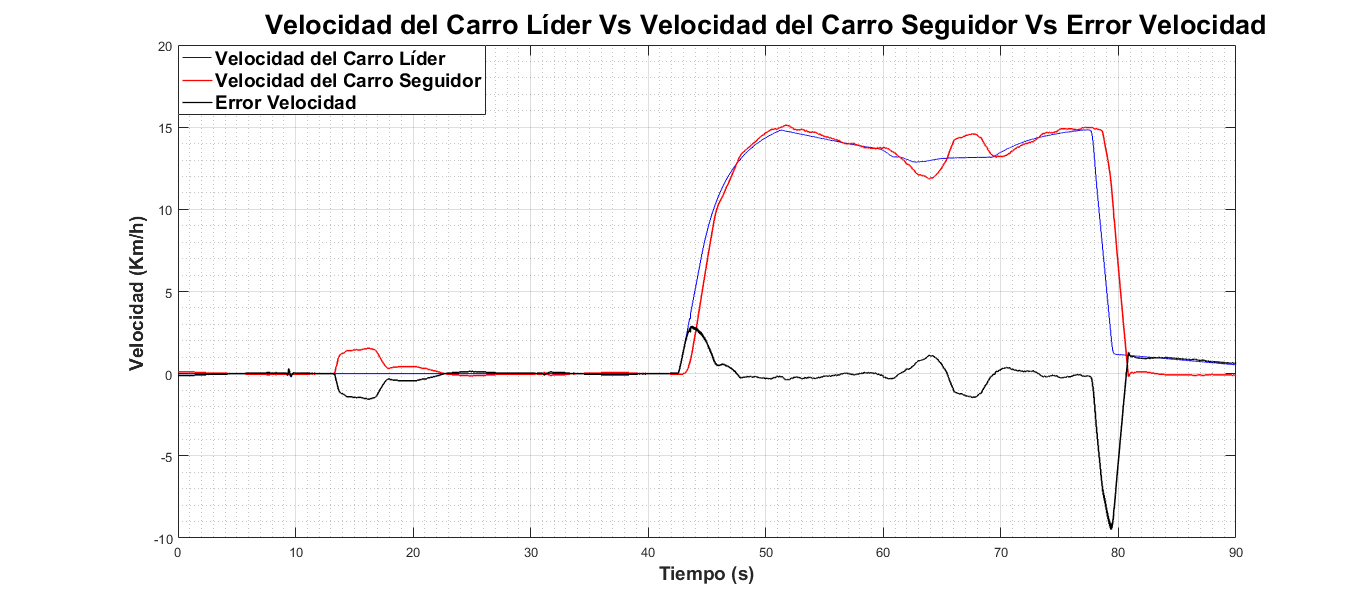
\includegraphics[scale=0.35]{Imagenes/velacccs}
		\caption{Gráfica de la velocidad de los vehículos}
		\label{fig:velacccs}
\end{figure}	

\begin{figure}[H]
	\centering
		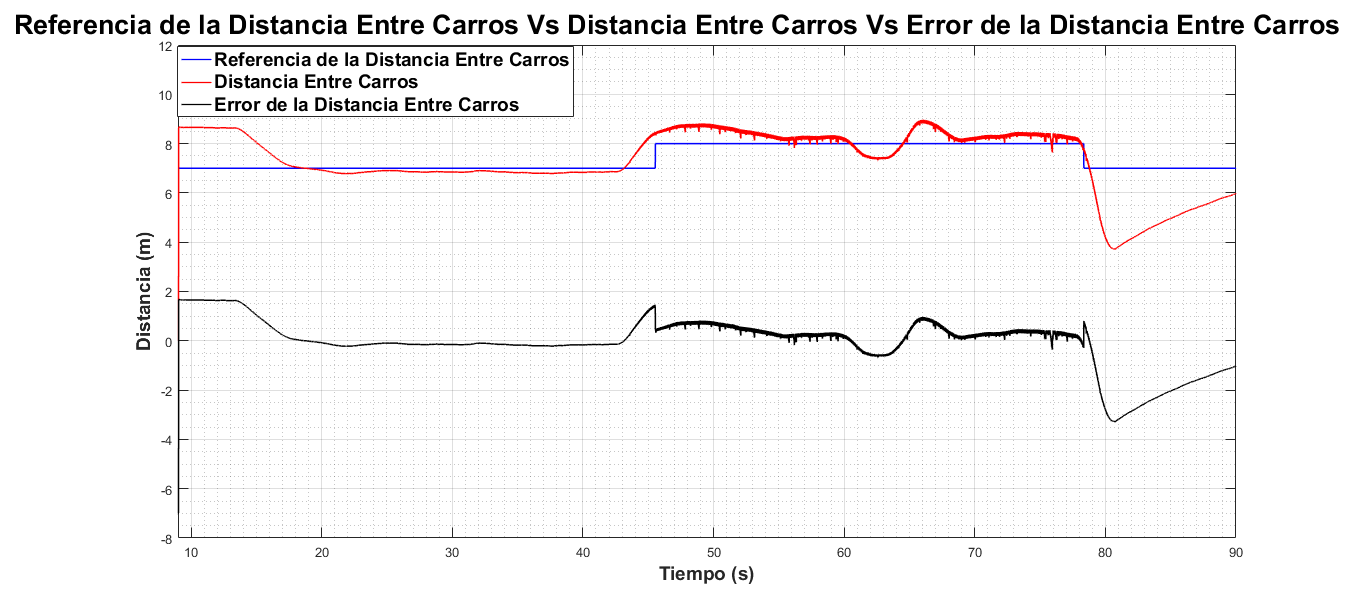
\includegraphics[scale=0.35]{Imagenes/distacccs}
		\caption{Gráfica del error de la distancia de los vehículos}
		\label{fig:distacccs}
\end{figure}	



%%%%%%
\subsection{\textit{Stop and Go}}
%%%%%%
Como se aprecia en la Figura \ref{fig:velstgcs}, el vehículo tardó 1 s más en arrancar, lo que implicó que, el error en la distancia (Figura \ref{fig:diststgcs}) aumentáse hasta 2 m por encima de la referencia, produciendo así, que se compensara aumanetando la velocidad. A raíz de este acontecimiento, el frenado se realizó 1 s más tarde, dejando al vehículo seguidor 1 m por debajo de la distancia de seguridad, error equivalente al 14 \%, valor que si bien puede ser mejorado, puede ser considerado como aceptable.\\   
\begin{figure}[H]
	\centering
		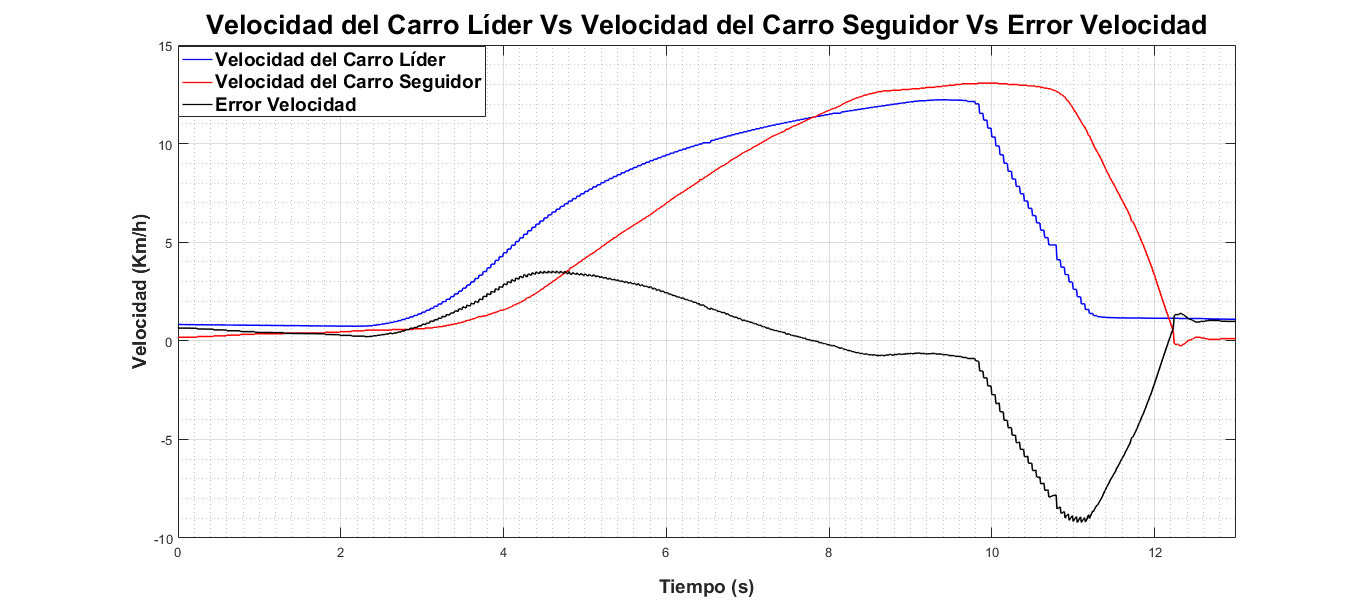
\includegraphics[scale=0.35]{Imagenes/velstgcs}
		\caption{Gráfica de la velocidad de los vehículos}
		\label{fig:velstgcs}
\end{figure}	

\begin{figure}[H]
	\centering
		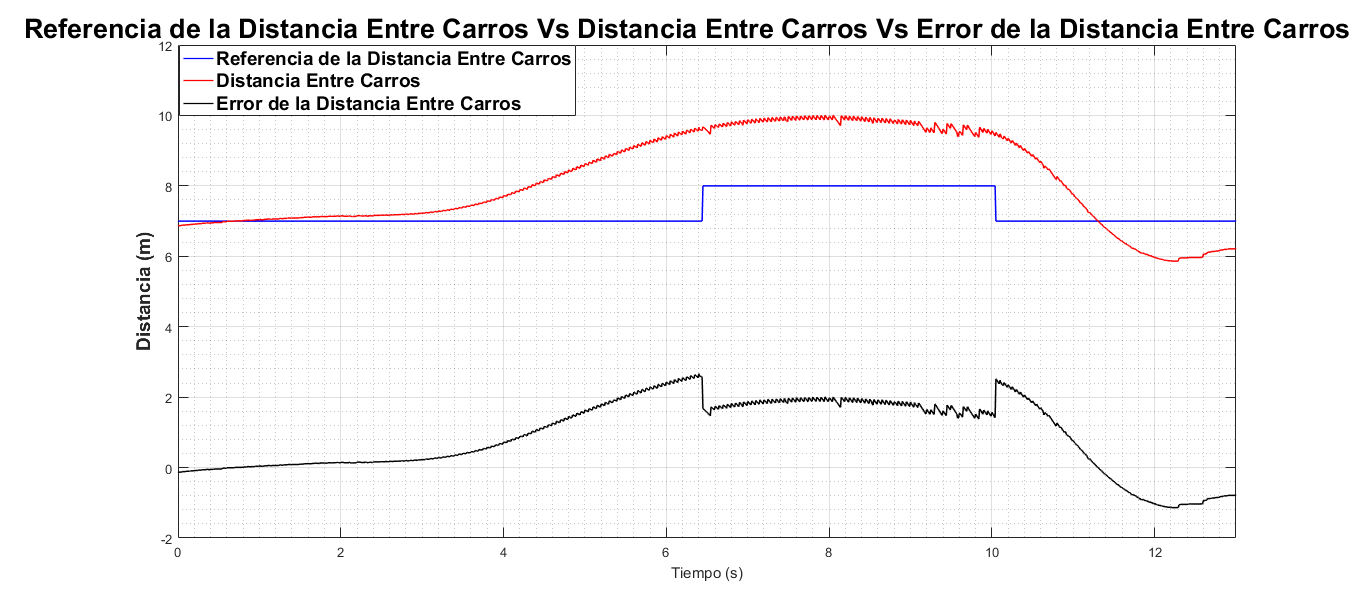
\includegraphics[scale=0.35]{Imagenes/diststgcs}
		\caption{Gráfica del error de la distancia de los vehículos}
		\label{fig:diststgcs}
\end{figure}	



\section{Resumen}

En el capítulo 7 se presentaron los resultados finales del trabajo, los cuales engloban el sistema de comunicaciones explicado en el capítulo 5 y las maniobras cooperativas descritas en el capítulo 6. En el mismo, se observan los tres escenearios planteados, comunicación PC - PC, V2V y Vehículo - PC, junto con sus debidas conisderaciones y pruebas.\\

\par Obteniendo, que en la comunicación PC - PC, los controladores se comportaron de la forma esperada, permitiendo que las maniobras se puedan ejecutar correctamente, sin que las comunicaciones presenten retrasos considerables. En la comunicación V2V, aunque fue la que presentó más errores, en la misma se pudo ejecutar las maniobras de forma correcta. Finalmente, la comunicación Vehículo - PC, siendo el caso con mayor complejidad arrojó buenos resultados, efectuándose las maniobras con bajo error, a excepción de algunos casos puntuales.